\documentclass[a4paper,10pt]{article}
\usepackage{fontspec}
\usepackage{setspace}
\usepackage{booktabs}
\usepackage{amsmath}
\usepackage{cancel}
\usepackage{graphicx}
\usepackage{biblatex}
\usepackage{float}

\setmainfont{arial}
\setstretch{1.15}
\addbibresource{references.bib}

\title{Activation Function and Forward Propagation}
\author{Arif Suganda\\
        Tadulako University\\
        \texttt{f5522530002@untad.ac.id}
}

\begin{document}
\maketitle

\section{Activation Function}
Activation function used in this assignment are ReLU for neurons located in the hidden layers and Sigmoid for neurons located in the output layer.
\subsection{ReLU}
ReLU function is defined as:
\begin{equation}
    \text{ReLU}(z) = \begin{cases}
    z & \text{if } z > 0 \\
    0 & \text{if } z \leq 0
    \end{cases}
\end{equation}
\noindent
The derivative of ReLU is:
\begin{equation}
    \text{ReLU}'(z) = \begin{cases}
    1 & \text{if } z > 0 \\
    0 & \text{if } z \leq 0
    \end{cases}
\end{equation}

\subsection{Sigmoid}
Sigmoid function is defined as:
\begin{equation}
    \sigma(z) = \frac{1}{1 + e^{-z}}
\end{equation}
The derivative of the sigmoid function is defined as:
\begin{equation}
    \sigma'(z) = \sigma(z)(1 - \sigma(z))
\end{equation}

\section{Implementation}

The implementation of the activation function and forward propagation is done using XOR gate problem.
Which is a non-linear problem that cannot be solved using a single layer perceptron. 
The architecture of the model can be seen in Figure \ref{fig:perceptron_xor_gate}.

\begin{figure}[H]
    \centering
    
\includegraphics[width=1\textwidth]{perceptron_xor_gate.png} 
    \caption{Diagram of 2 Layers Perceptron XOR Gate}\label{fig:perceptron_xor_gate}
\end{figure}

The model consists of 2 input neurons, 4 hidden layer neurons using ReLU activation function, and 1 output neuron using Sigmoid activation function.
The training process is done for 1000 epochs with a learning rate of 0.1.
The reason for the hidden layer using 4 neurons is due to the dying ReLU problem which often occurs during the previous training process using 2 hidden layer neurons.

\subsection{Code}

\textbf{Import}
\begin{verbatim}
import matplotlib.pyplot as plt
import numpy as np
\end{verbatim}

\noindent
\textbf{Sigmoid}
\begin{verbatim}
def sigmoid(z):
    return 1 / (1 + np.exp(-z))

def sigmoid_derivative(z):
    s = sigmoid(z)
    return s * (1 - s)
\end{verbatim}

\noindent
\textbf{Relu}
\begin{verbatim}
def relu(z):
    return np.maximum(0, z)

def relu_derivative(z):
    return (z > 0).astype(float)
\end{verbatim}

\noindent
\textbf{Training}
\begin{verbatim}
def train(X, y, layers, epochs=1000, lr=0.1):
    n_layers = len(layers)
    i_bias = 1
    i_weight = 0
    histories = []
    
    activation_functions_history = []
    
    for i in range(epochs):
        # Forward
        current_input = X
        layers_output = [X]
        layers_sum = [X]
        
        for (i, layer) in enumerate(layers):
            current_sum = calculate_sum(
                current_input, layer[i_weight], layer[i_bias])
            if i == n_layers - 1:
                current_input = sigmoid(current_sum)
            else:
                current_input = relu(current_sum)
            layers_sum.append(current_sum)
            layers_output.append(current_input)
        
        activation_functions_history.append(
            [layers_sum, layers_output])

        # Backpropagation
        d_layers_output = []
        
        # Loss function and output layer delta
        delta = calculate_delta(y, layers_output[-1])
        print(f"Epoch {i+1}/{epochs}, Loss: {calculate_loss(y, 
        layers_output[-1]):.4f}")
        d_layers_output.append(delta)
        
        # Hidden layer propagation
        for j in range(n_layers - 1, 0, -1):
            weight = delta.dot(layers[j][i_weight].T)
            delta = weight * relu_derivative(layers_sum[j])
            d_layers_output.append(delta)
        d_layers_output.reverse()
        
        # Update weight
        for j in range(n_layers):
            layer_input = layers_output[j]
            delta_j = d_layers_output[j]
            
            layers[j][i_weight] -= layer_input.T.dot(
                delta_j) * lr
            layers[j][i_bias] -= np.sum(
                delta_j, axis=0, keepdims=True) * lr
        
        histories.append(
            [ [w.copy(), b.copy()] for w, b in layers ])
        
    return activation_functions_history, histories, layers
\end{verbatim}

\noindent
\textbf{Prediction}
\begin{verbatim}
def predict(X, layers):
    i_bias = 1
    i_weight = 0
    input_x = X
    for (j, layer) in enumerate(layers):
        current_sum = calculate_sum(
            input_x, layer[i_weight], layer[i_bias])
        if j == len(layers) - 1:
            input_x = sigmoid(current_sum)
        else:
            input_x = relu(current_sum)
    return input_x
\end{verbatim}

\noindent
\textbf{Run}
\begin{verbatim}
n_input_neurons = 2
n_hidden_neurons = 4
n_output_neurons = 1

layers = []

w_hidden = np.random.uniform(
    size=(n_input_neurons, n_hidden_neurons))
b_hidden = np.zeros((1, n_hidden_neurons))
layers.append([w_hidden, b_hidden])

w_out = np.random.uniform(
    size=(n_hidden_neurons, n_output_neurons))
b_out = np.zeros((1, n_output_neurons))
layers.append([w_out, b_out])

X = np.array([[0,0], [0,1], [1,0], [1,1]])
y = np.array([[0], [1], [1], [0]])

activation_functions_history, histories, model = train(
    X, y, layers)

print("Predictions after training:")
predictions = predict(X, model)
for i in range(len(X)):
    print(f"""Input: {X[i]} -> 
    Predicted: {predictions[i][0]:.4f} to 
    {1 if predictions[i][0] > 0.5 else 0}""")
\end{verbatim}

\noindent
\textbf{Result}

\begin{figure}[H]
    \centering
    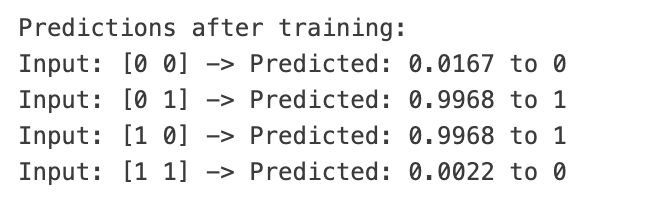
\includegraphics[width=0.8\textwidth]{result_training.png} 
    \caption{Training result}\label{fig:result_training}
\end{figure}

\noindent
\textbf{Filter ReLU and Sigmoid activation and output}
\begin{verbatim}
reduction = -60
iteration = 1000
n_sample = (iteration / abs(reduction)) * (
    len(X) * n_hidden_neurons)

relu_sum = np.array([])
relu_activation = np.array([])
sigmoid_sum = np.array([])
sigmoid_activation = np.array([])
for i in range(len(activation_functions_history) -1, 
    len(activation_functions_history) - iteration - 1, 
    reduction):
    relu_sum = np.append(
        relu_sum, 
        np.array(activation_functions_history[i][0][1]))
    relu_activation = np.append(
        relu_activation, 
        np.array(
            activation_functions_history[i][1][1]).flatten())
    sigmoid_sum = np.append(
        sigmoid_sum,
        np.array(
            activation_functions_history[i][0][2]))
    sigmoid_activation = np.append(
        sigmoid_activation, 
        np.array(
            activation_functions_history[i][1][2]).flatten())
\end{verbatim}

\noindent
\textbf{Show ReLU samples}
\begin{verbatim}
relu_maps = np.vstack((relu_sum, relu_activation))

plt.figure(figsize=(8, 5))
plt.scatter(relu_maps[0, :], 
relu_maps[1, :], color='blue', label='Neurons')

# Adding Cartesian axes for clarity
plt.axhline(0, color='black', linewidth=1) # X-axis
plt.axvline(0, color='black', linewidth=1) # Y-axis

plt.title(f"ReLU Activations ({n_sample:.0f} Samples)")
plt.xlabel("Input (z)")
plt.ylabel("Output (a)")
plt.grid(True, linestyle='--', alpha=0.6)
plt.legend()
plt.show()
\end{verbatim}

\noindent
\textbf{ReLU samples}
\begin{figure}[H]
    \centering
    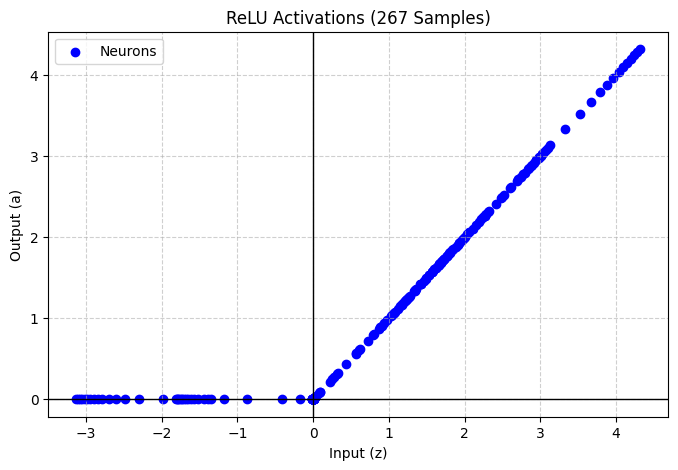
\includegraphics[width=1\textwidth]{relu_samples.png} 
    \caption{ReLU samples}\label{fig:relu_samples}
\end{figure}

\noindent
\textbf{Show Sigmoid samples}
\begin{verbatim}
sigmoid_maps = np.vstack(
    (sigmoid_sum, sigmoid_activation))

plt.figure(figsize=(8, 5))
plt.scatter(
    sigmoid_maps[0, :], 
    sigmoid_maps[1, :], 
    color='blue', 
    label='Neurons')

# Adding Cartesian axes for clarity
plt.axhline(0, color='black', linewidth=1) # X-axis
plt.axvline(0, color='black', linewidth=1) # Y-axis

plt.title(f"""Sigmoid Activations 
({n_sample:.0f} Samples)""")
plt.xlabel("Input (z)")
plt.ylabel("Output (a)")
plt.grid(True, linestyle='--', alpha=0.6)
plt.legend()
plt.show()
\end{verbatim}

\noindent
\textbf{Sigmoid samples}
\begin{figure}[H]
    \centering
    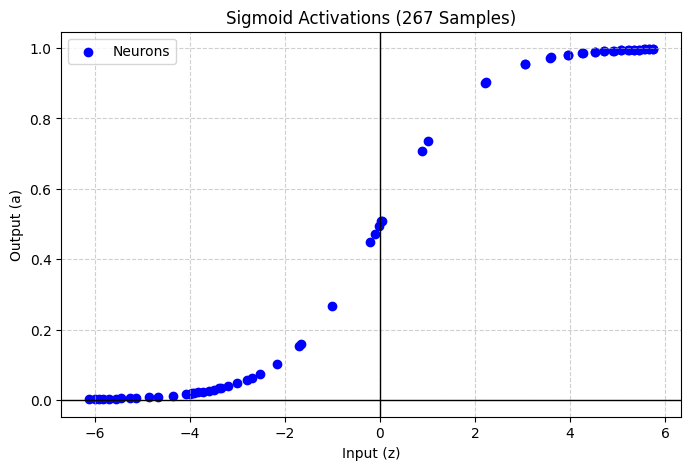
\includegraphics[width=1\textwidth]{sigmoid_samples.png} 
    \caption{Sigmoid samples}\label{fig:sigmoid_samples}
\end{figure}

\section{Forward Propagation}

Neural network for this forward propagation can be seen in Figure~\ref*{fig:perceptron_xor_gate} and input can be seen in Table~\ref*{tab:xor_gate}.
\begin{table}[h]
    \centering
    \caption{Truth Table for XOR Gate}\label{tab:xor_gate}
    \begin{tabular}{c c c}
        \toprule
        \textbf{Input A} & \textbf{Input B} & \textbf{Output (A + B)} \\
        \midrule
        0 & 0 & 0 \\
        0 & 1 & 1 \\
        1 & 0 & 1 \\
        1 & 1 & 0 \\
        \bottomrule
    \end{tabular}
\end{table}

\noindent
\textbf{Input 1}
$X_1 = 0, X_2 = 0$
\begin{align*}
\intertext{$ReLU_{11}$ calculation}
    z_{11} &= w_{111} x_1 + w_{112} x_2 + b_{11} \\
    z_{11} &= 1.74299359 * 0 + -1.74294969 * 0 + (3.27671157e-04) \\
    z_{11} &= 3.27671157e-04 \\
    \sigma(z_{11}) &= \begin{cases}
    z & \text{if } z > 0 \\
    0 & \text{if } z \leq 0
    \end{cases} \\
    \sigma(z_{11}) &= 3.27671157e-04 
\intertext{$ReLU_{12}$ calculation}
    z_{12} &= w_{121} x_1 + w_{122} x_2 + b_{12} \\
    z_{12} &= 2.94345231 * 0 + -2.94335356 * 0 + (-1.80455814e-04) \\
    z_{12} &= -1.80455814e-04 \\
    \sigma(z_{12}) &= \begin{cases}
    z & \text{if } z > 0 \\
    0 & \text{if } z \leq 0
    \end{cases} \\
    \sigma(z_{12}) &= 0
\intertext{$ReLU_{13}$ calculation}
    z_{13} &= w_{131} x_1 + w_{132} x_2 + b_{13} \\
    z_{13} &= 1.53434956 * 0 + -1.23643017 * 0 + (1.78022709e+00) \\
    z_{13} &= 1.78022709e+00 \\
    \sigma(z_{13}) &= \begin{cases}
    z & \text{if } z > 0 \\
    0 & \text{if } z \leq 0
    \end{cases} \\
    \sigma(z_{13}) &= 1.78022709e+00
\intertext{$ReLU_{14}$ calculation}
    z_{14} &= w_{141} x_1 + w_{142} x_2 + b_{14} \\
    z_{14} &= -2.53376151 * 0 + 2.53434076 * 0 + (-2.94107741e-04) \\
    z_{14} &= -2.94107741e-04 \\
    \sigma(z_{14}) &= \begin{cases}
    z & \text{if } z > 0 \\
    0 & \text{if } z \leq 0
    \end{cases} \\
    \sigma(z_{14}) &= 0
\intertext{$Sigmoid_{21}$ calculation}
    z_{21} &= w_{211} ReLU_{11} + w_{212} ReLU_{12} + w_{213} ReLU_{13} + w_{214} ReLU_{14} + b_{21} \\
    z_{21} &= 2.47460371 * 3.27671157e-04 \\
    &\quad + 4.07719726 * 0 + (-2.55047176) * 1.78022709 \\
    &\quad + 3.55494981 * 0 + (-1.27403197) \\
    z_{21} &= -5.81364005 \\
    \sigma(z_{21}) &= \frac{1}{1 + e^{-(-5.81364005)}} \\
    \sigma(z_{21}) &= 0.002
\intertext{$\hat{y}$ calculation}
    \hat{y} &= \begin{cases}
        1 & \text{if } \sigma_{21} \ge 0.5 \\
        0 & \text{if } \sigma_{21} < 0.5
    \end{cases}\\
    \hat{y} &= 0
\end{align*}

\noindent
\textbf{Input 2}
$X_1 = 0, X_2 = 1$
\begin{align*}
\intertext{$ReLU_{11}$ calculation}
    z_{11} &= w_{111} x_1 + w_{112} x_2 + b_{11} \\
    z_{11} &= 1.74299359 * 0 + -1.74294969 * 1 + (3.27671157e-04) \\
    z_{11} &= -1.74262202e+00 \\
    \sigma(z_{11}) &= \begin{cases}
    z & \text{if } z > 0 \\
    0 & \text{if } z \leq 0
    \end{cases} \\
    \sigma(z_{11}) &= 0
\intertext{$ReLU_{12}$ calculation}
    z_{12} &= w_{121} x_1 + w_{122} x_2 + b_{12} \\
    z_{12} &= 2.94345231 * 0 + -2.94335356 * 1 + (-1.80455814e-04) \\
    z_{12} &= -2.94353402e+00 \\
    \sigma(z_{12}) &= \begin{cases}
    z & \text{if } z > 0 \\
    0 & \text{if } z \leq 0
    \end{cases} \\
    \sigma(z_{12}) &= 0
\intertext{$ReLU_{13}$ calculation}
    z_{13} &= w_{131} x_1 + w_{132} x_2 + b_{13} \\
    z_{13} &= 1.53434956 * 0 + -1.23643017 * 1 + (1.78022709e+00) \\
    z_{13} &= 5.43796917e-01 \\
    \sigma(z_{13}) &= \begin{cases}
    z & \text{if } z > 0 \\
    0 & \text{if } z \leq 0
    \end{cases} \\
    \sigma(z_{13}) &= 5.43796917e-01
\intertext{$ReLU_{14}$ calculation}
    z_{14} &= w_{141} x_1 + w_{142} x_2 + b_{14} \\
    z_{14} &= -2.53376151 * 0 + 2.53434076 * 1 + (-2.94107741e-04) \\
    z_{14} &= 2.53404665e+00 \\
    \sigma(z_{14}) &= \begin{cases}
    z & \text{if } z > 0 \\
    0 & \text{if } z \leq 0
    \end{cases} \\
    \sigma(z_{14}) &= 2.53404665e+00
\intertext{$ReLU_{21}$ calculation}
    z_{21} &= w_{211} ReLU_{11} + w_{212} ReLU_{12} + w_{213} ReLU_{13} + w_{214} ReLU_{14} + b_{21} \\
    z_{21} &= 2.47460371 * 0 \\
    &\quad + 4.07719726 * 0 + (-2.55047176) * 5.43796917e-01 \\
    &\quad + 3.55494981 * 2.53404665e+00 + (-1.27403197) \\
    z_{21} &= 6.34743799 \\
    \sigma(z_{21}) &= \frac{1}{1 + e^{-(6.34743799)}} \\
    \sigma(z_{21}) &= 0.998
\intertext{$\hat{y}$ calculation}
    \hat{y} &= \begin{cases}
        1 & \text{if } \sigma_{21} \ge 0.5 \\
        0 & \text{if } \sigma_{21} < 0.5
    \end{cases}\\
    \hat{y} &= 1
\end{align*}

\end{document}